% vim:ft=tex:
%
\documentclass[12pt]{article}
\usepackage[margin=1in]{geometry}
\usepackage{graphicx}
\usepackage{enumitem}

% Bibliography
\usepackage[backend=bibtex,firstinits=true,style=ieee]{biblatex}
\AtEveryBibitem{%
  \clearname{translator}%
  \clearlist{publisher}%
  \clearlist{address}%
  \clearlist{location}%
  \clearfield{pagetotal}%
  \clearfield{isbn}%
  \clearfield{url}%
  \clearfield{doi}%
  \clearfield{series}%
  \clearfield{language}%
  \clearfield{pages}%
  \clearfield{volume}%
  \clearfield{urlday}%
  \clearfield{urlmonth}%
  \clearfield{urlyear}%
  \clearfield{issn}%
  \clearname{editor}%
}
\addbibresource{references}

\begin{document}

\pagenumbering{gobble}

\begin{center}
  \textbf{Interaction Patterns for Mixed Initiative Exploration of a Parameter Space \\
  with an ``Active Learner'' Fabrication Machine}\\
  \vspace{.5em}
  Andrew Head
\end{center}

As you enter the Invention Lab, Berkeley's student hackerspace, you notice  that working with fabrication machines is hard.
Scorched cardboard sits atop the scrap pile from laser cuts that caught fire.
Failed 3D prints line the foyer walls, deformed from thin supports or improper orientation.
% As you walk into the foyer of Berkeley's student hackerspace, you see dozens of failed 3D prints lined up along the walls.
% These tell a solemn truth:
% Getting started with fabrication hardware is hard.
% 3D printing without large enough tolerances leaves movable parts stationary.
% Thin supports or sharp overhangs result in tangled spindles of ABS that fail to layer properly.
%When using a laser cutter, vector cutting with the power set too high lights the workpiece on fire.
This work seeks to \textbf{improve the efficiency and effectiveness of early, exploratory interactions with fabrication machines.}

I will focus improving the user experience of of rastering images onto arbitrary materials using a laser cutter.
Rastering is the process of ``etching'' an image into a work piece with with a dot matrix of laser fixations.
Four parameters---power, speed, frequency, and resolution---control the depth, speed, and fidelity of the image is rastered (Figure~\ref{fig:rasters}).
Many values for these parameters can cause the material to scorch.

The proposed research aims for a vision for fabrication machines that will be able to assist users in helping them to learn their parameters, models of operation, and constraints.
I propose that a laser cutter that follows active learning can help a user more efficiently explore the space of possible parameters and converge on an optimal set of parameters.
The intended contributions of this work are:
\begin{enumerate}[noitemsep]
\item A catalog of user problems actualizing their design intent with laser cutters
\item Application of active learning to discovering an ideal fabrication machine configuration
\item A qualitative and quantitative comparison of guided exploration of the configuration space to trial-and-error approaches
\end{enumerate}

%  \item How can a robot learn an ideal configuration for a task without demonstrations?
%   \item What are the most efficient subjective inputs and interaction techniques to enable fast convergence to an ideal configuration with a fabrication machine?

% for a new material, or to systematically vary these parameters until a raster.
% The values of these are vary based on the material a user is working with, the speed they want to work to get done with, the depth of the marks, and how rough of a sketch they can accept for the current raster.
% A major failure occurs in that the hacker will likely want to use the machine long before they want to develop an accurate mental model of how the parameters impact the work to be done.

% There is no clear way how learning from demonstration techniques can be used to describe configurations for settings such as laser power, speed, frequency, and resolution.
% Furthermore, these parameters don't map directly to the task the user wants to perform.
% The hacker may have a clear idea of the appearance of the material surface that they want to attain, and an understanding of how these parameters cause it just is not clear.

% This work aims to answer the following questions that, to my knowledge, are open questions within both the fields of human-robot interaction and the fabrication concentration of human-computer interaction.

This study will begin with a small number of interviews of with student members of the Invention Lab (around $n=5$).
Participants will be asked about the frequency, severity, and types of errors students encounter enacting their designs with a laser cutter.

I will implement an active learning algorithm for guiding a user to discover the ideal configuration for rastering an image with a laser cutter (for background, see~\cite{settles_active_2010}).
The algorithm will provide examples to a user in order to collect an \emph{ordinal} rating of example quality.
Each example will be a machine configuration including laser power, speed, frequency, and resolution.
As we are attempting to discover some function that predicts configuration quality in the pursuit of some optimal configuration, I will implement the algorithm based on past work that discovers models that predict continuous values (e.g.~\cite{sugiyama_active_2008}).
% Currently, I suspect that a Gaussian kernel function or a quadratic curve will best express a user's perception of the quality of a configuration in actualizing their design.

To understand the benefits and disadvantages of mixed initiative parameter space exploration based on active learning, I will run a usability study.
Participants will be asked to reproduce laser cut raster jobs based on workpieces I provide.
Method of parameter exploration will be varied:
in one condition, they will lead themselves to find the ideal parameters.
In the other, participants will be led through exploration of the configuration space by the active learning algorithm.
I will measure the number of configurations tested 
I will also ask Likert scale questions about perceptions of difficulty and satisfaction with each method of system, and ask for qualitative feedback.

The usability study will be run in the Invention Lab with the Universal Laser Systems VLS3.50 machine.
I have received clearance to work with this equipment.
Given the limits of the hardware available, the initial proposed study will likely include around 4--6 testers altogether.
% Measurements collected will include the time and iterations taken to perform the task, Likert scale ratings of user satisfaction, and qualitative feedback about strategies to achieve the ideal rastering.

\begin{figure}
  \centering
  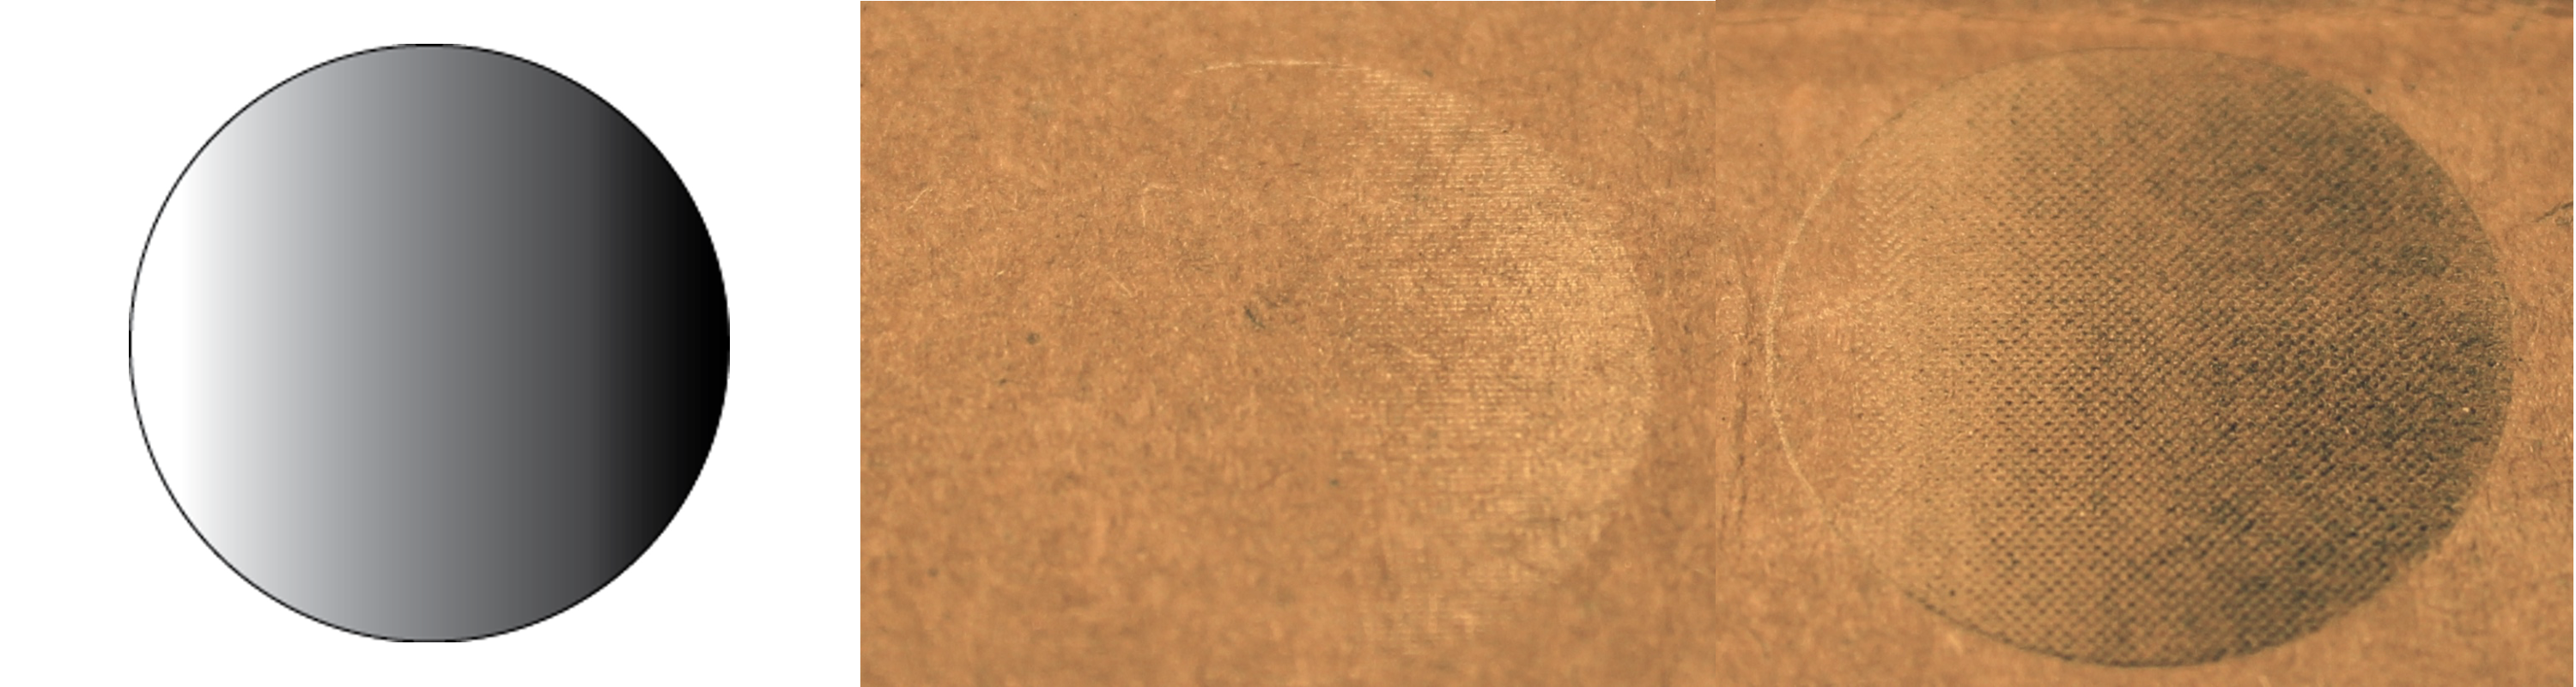
\includegraphics[width=0.6\textwidth]{figures/rasters}
  \caption{\small{%
  A drawing `rastered' into cardboard by a laser cutter with two different configurations.
  \emph{Left}: the original image given to the laser cutter.
  \emph{Center}: an etching that is too faint to see due to low power.
  \emph{Right}: an etching that scorched the cardboard due to high power and low speed.
  A user of the laser cutter will have to manipulate the laser's parameters to get the desired appearance.}}
\label{fig:rasters}
\end{figure}

\printbibliography[heading=none]

\end{document}
